% Verbatim from minor_report/chapters/chapter_4_results.tex lines 1043-1110 (retired report),
% headings demoted by 0 level(s). Do not edit here; edit the source of the numbers.

Table~\ref{tab:anomaly-catalogue} records anomalous behaviour visible in the
logs and derived metrics. It deliberately separates observation from causal
explanation: no item below identifies a root cause, and the possible mechanisms
listed in the analysis catalogue remain untested.

\begingroup
\small
\setlength{\tabcolsep}{4pt}
% longtable captions default to 4in, which sets this one in a narrow indented
% block instead of across the table.
\setlength{\LTcapwidth}{\textwidth}
% Column widths plus 8 inter-column gaps must not exceed \textwidth, or the
% table is set into the right margin.
\begin{longtable}{p{0.05\textwidth}p{0.10\textwidth}p{0.26\textwidth}p{0.50\textwidth}}
\caption[Anomaly catalogue for the relogged campaign.]{Anomaly catalogue for the relogged campaign. Severity prioritizes
impact on interpretation, not certainty about cause.}
\label{tab:anomaly-catalogue}\\
\toprule
ID & Severity & Observation & Quantitative evidence and reporting consequence \\
\midrule
\endfirsthead
\toprule
ID & Severity & Observation & Quantitative evidence and reporting consequence \\
\midrule
\endhead
A1 & Critical & Requested VINS+YOLO filtering was inactive & All 12 folders contain
28,038 mask rows in total, but zero matched detector messages, positive-box
rows, or nonzero-coverage rows. They cannot measure an active semantic-filter
treatment. \\
A2 & High & ORB+YOLO exposure varied between repeats & Positive-box fractions
range from 1.4\% to 99.2\%, including wide variation among repeats of the same
bag. A matched detector message can contain zero boxes, so match count alone is
not treatment dose. \\
A3 & Critical & Every dynamic trajectory contains discontinuities & All 48
dynamic runs contain impossible-speed steps. Median affected-step fractions are
59.6\% (VINS), 30.3\% (ORB), 61.1\% (requested VINS+YOLO), and 26.9\%
(ORB+YOLO). Global ATE cannot be read as ordinary drift. \\
A4 & High & Global and clean-segment errors are strongly separated & Median
global-to-clean ATE ratios are 100, 146, 101, and 239 respectively. Locally
coherent intervals coexist with catastrophic full-run discontinuities. \\
A5 & Medium & Static ORB has an isolated initialization-adjacent jump & All nine
static ORB runs have one or two jumps, with the first near 2.6~s. Where an
inertial transition timestamp exists, the jump precedes it by 0.10--0.17~s;
this temporal association does not establish causation. \\
A6 & Medium & Two ORB run summaries are incomplete & The two static repeat
summaries omit final inertial/map fields, although frame and local-mapping logs
record initialized operation. Summary-only validation would falsely exclude
these runs. \\
A7 & High & ORB baseline/filter inputs are not paired in 11 of 12 cases & Invalid
pairs differ in received-frame count by 9.95--30.06\%, while their durations
differ by less than 0.13\%. Most between-mode differences are descriptive, not
controlled treatment effects. \\
A8 & Medium & VINS reset counts are non-discriminating & All 33 VINS baseline
and requested-filter runs have failure detection disabled and record zero
resets. Zero resets therefore cannot establish healthy estimation. \\
\bottomrule
\end{longtable}
\endgroup

\begin{figure}[htbp]
  \centering
  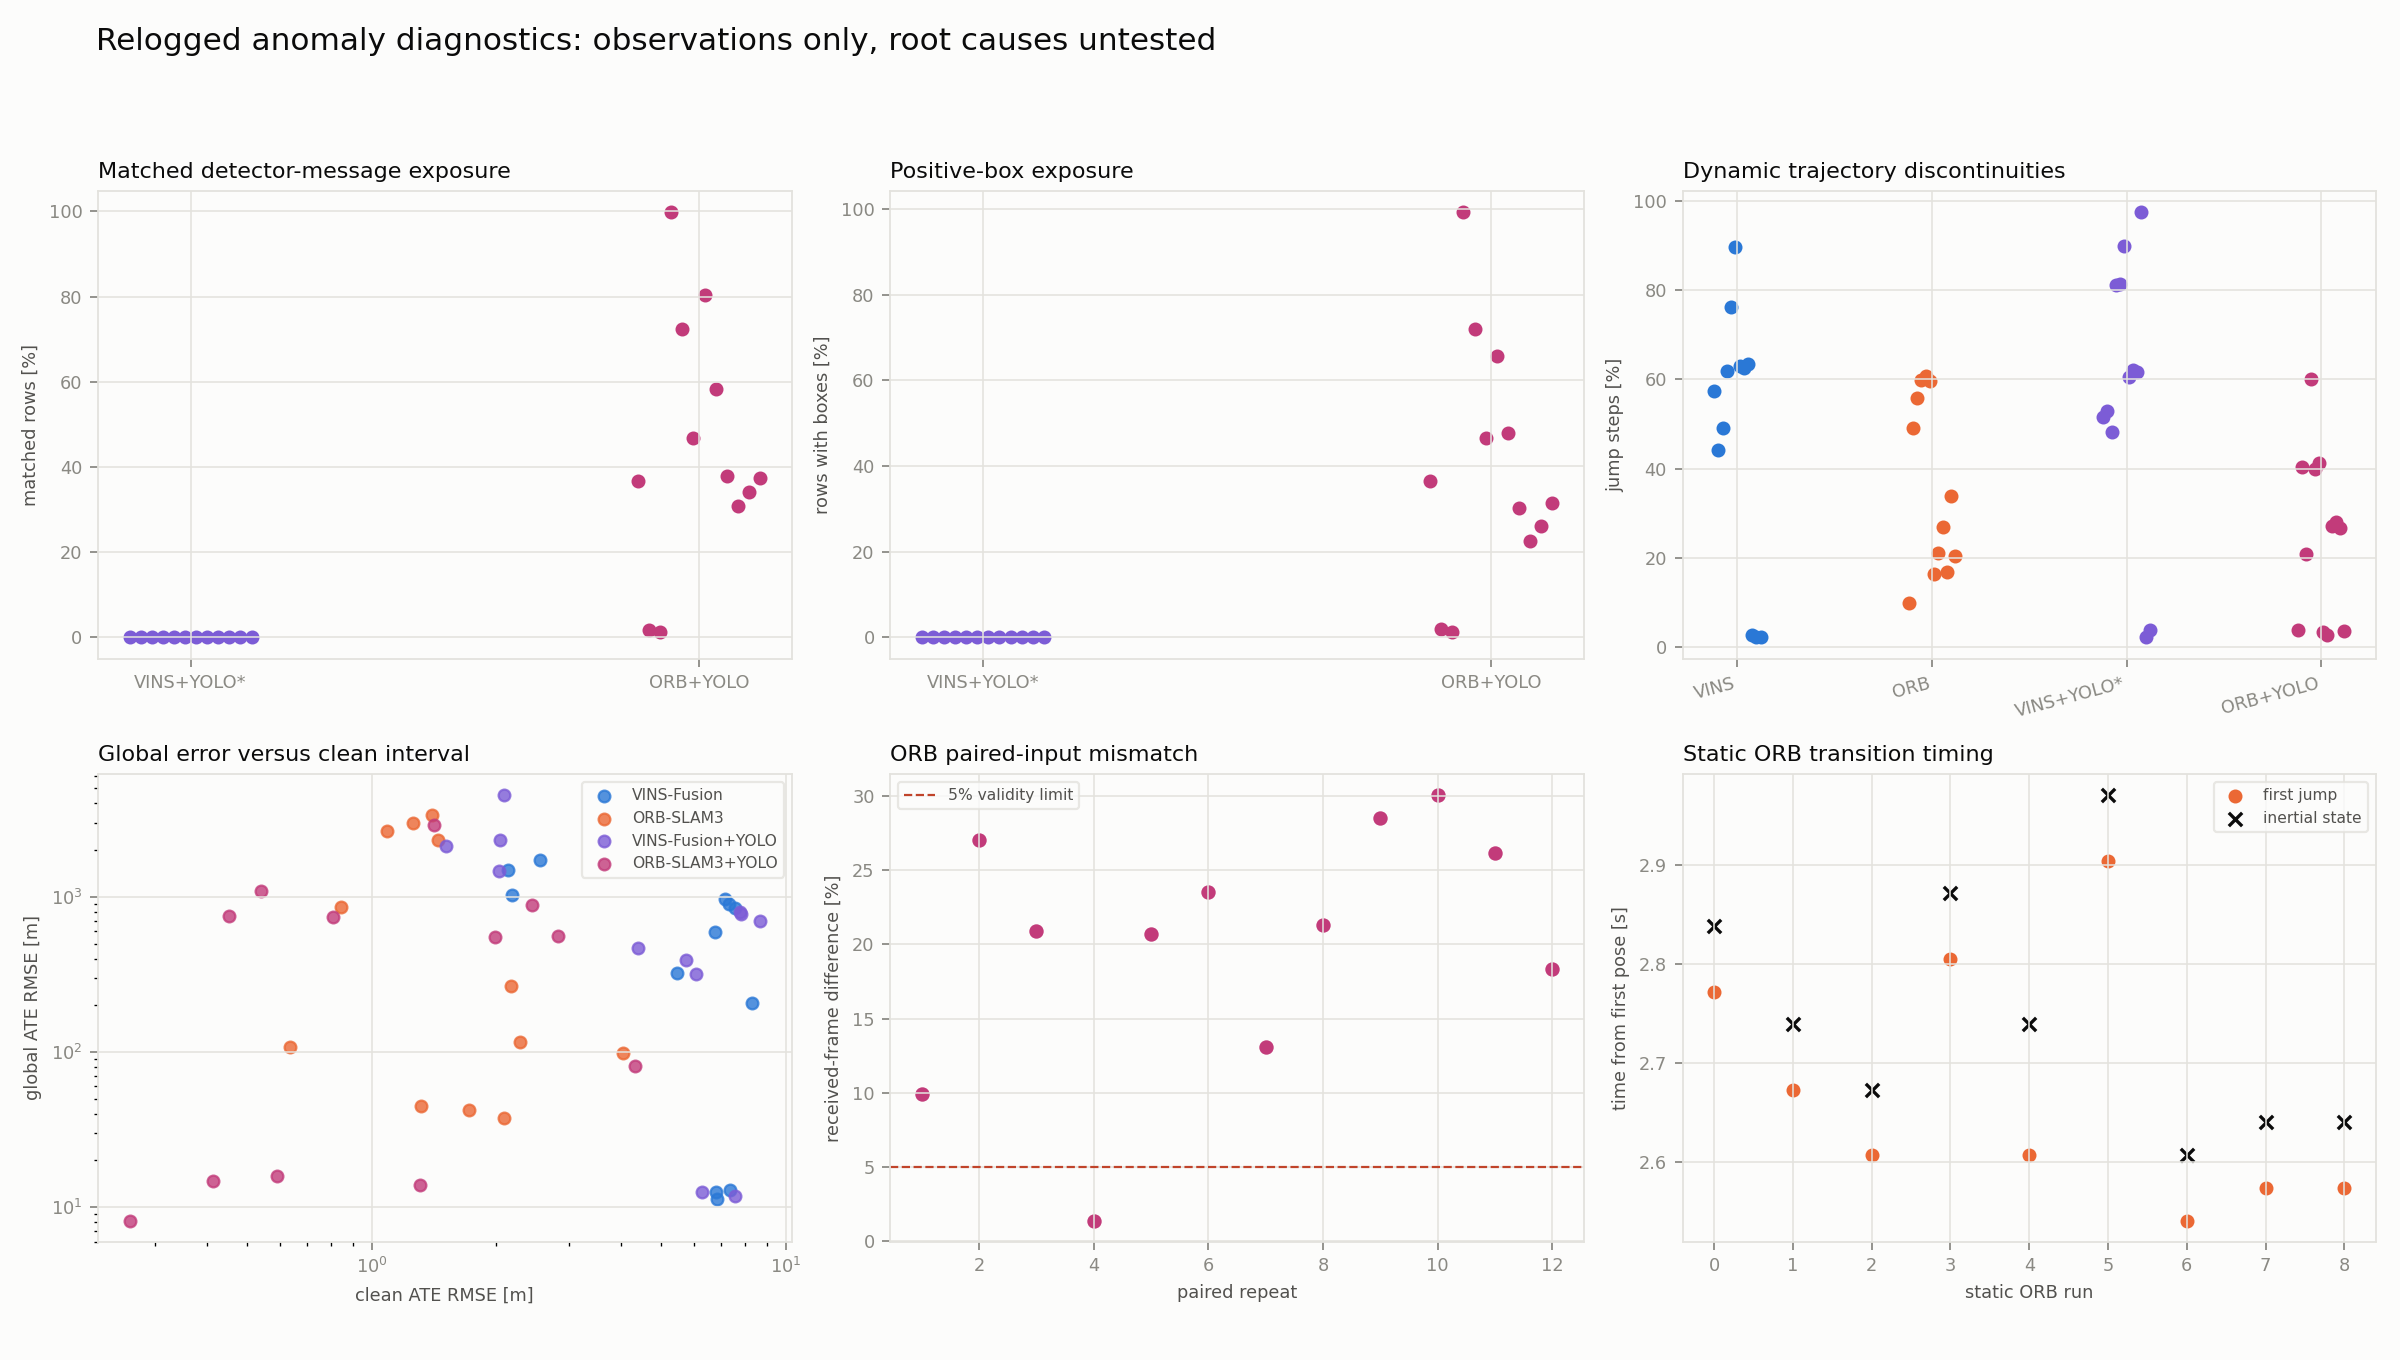
\includegraphics[width=\textwidth]{../../../output/compare/relogged_20260916/anomaly_diagnostics_light.png}
  \caption[Run-level anomaly diagnostics.]{Run-level anomaly diagnostics. The panels show detector-message and
  positive-box exposure, dynamic jump fractions, global versus clean-segment
  ATE, ORB paired-input mismatch, and static ORB jump timing. These are
  observations only; the plot does not assign a root cause.}
  \label{fig:anomaly-diagnostics}
\end{figure}
